\documentclass[conference]{IEEEtran}
\usepackage{luatexja}
\usepackage{amsmath,amssymb}
\usepackage{booktabs}
\usepackage{graphicx}
\usepackage{xcolor}
\usepackage{tikz}
\usetikzlibrary{arrows.meta,positioning,fit,backgrounds,calc}
\usepackage{float}
\usepackage{balance}
\usepackage[hidelinks]{hyperref}
\hypersetup{
  pdftitle={NinaXander：共有潜在表現による異種モデル族の凍結言語モデル合成――成立条件と限界},
  pdfauthor={樹神 宇徳,林 俊一郎,椋木 大地,星野 哲也,片桐 孝洋},
  pdfsubject={凍結したRWKVとTransformerの共有潜在表現による合成},
  pdfkeywords={language model composition, RWKV, Transformer, representation alignment}
}

\newcommand{\PH}[1]{{\color{red}\textbf{[#1]}}}
\newcommand{\kw}[1]{\textbf{#1}}
\newcommand{\Rsq}{R^2}
\newcommand{\RWKVself}{\textsf{RWKV自己再構成}}
\newcommand{\Pythiaself}{\textsf{Pythia自己再構成}}
\newcommand{\RtoP}{\textsf{RWKV$\to$Pythia}}
\newcommand{\PtoR}{\textsf{Pythia$\to$RWKV}}
\newcommand{\RtoPL}[1]{\RtoP{}（$L{=}#1$）}
\newcommand{\PtoRL}[1]{\PtoR{}（$L{=}#1$）}
\newcommand{\hfrepo}[2]{%
  \href{#1}{%
    \texttt{https://huggingface.co/kotama7/}\allowbreak\texttt{#2}}}
\newcommand{\hfcollection}[2]{%
  \href{#1}{%
    \texttt{https://huggingface.co/collections/kotama7/}\allowbreak\texttt{#2}}}

\title{\bfseries NinaXander：共有潜在表現による異種モデル族の凍結言語モデル合成――成立条件と限界}
\author{%
\IEEEauthorblockN{樹神 宇徳\IEEEauthorrefmark{1}，林 俊一郎\IEEEauthorrefmark{1}，
椋木 大地\IEEEauthorrefmark{2}，星野 哲也\IEEEauthorrefmark{2}，片桐 孝洋\IEEEauthorrefmark{2}}
\IEEEauthorblockA{\IEEEauthorrefmark{1}名古屋大学大学院情報学研究科}
\IEEEauthorblockA{\IEEEauthorrefmark{2}名古屋大学情報基盤センター}}

\begin{document}
\maketitle

\begin{abstract}
\kw{NinaXander} は，異なる事前学習系統の凍結層を，共有潜在アダプタを介して接続する言語モデルである。本研究では，
RWKV-4-Raven-7B（再帰型）と Tulu-Pythia-6.9b（Transformer 型）を対象に，対応層間の表現が単純な変換で接続可能か，
またその接続が機能的な合成に使えるかを検証する。主な結果は四つである。
\emph{(i)} 同一トークナイザ・幅・層数・学習領域という条件下で，中心化潜在相関
$\rho_{\mathrm{ctr}}{=}0.901$ を得た。行対応をシャッフルすると整合は消失する一方，生表現の CKA は同一層で最大にならず，
WikiText への領域シフトでも性能が大きく低下する。したがって，本結果が示すのは一般的な意味空間ではなく，
好条件下で学習可能なトークン対応表現である。
\emph{(ii)} 四経路の読み出しは \RWKVself{}／\RtoP{}／\Pythiaself{}／\PtoR{} の順に
$0.695/0.559/0.711/0.590$ であり，圧縮を除いても再構成誤差が残る。
\emph{(iii)} 最良直接アフィン写像は \RtoP{}／\PtoR{} で $0.487/0.535$ に達する一方，
学習済みアダプタ出力の $13.4\%/12.0\%$ はアフィン写像で説明できない。同一アダプタの
非線形枝を無効化すると両横断読み出しは負の $\Rsq$ まで崩れる。
\emph{(iv)} 単一境界で合成したキメラは構文的に妥当な生成と多肢選択の遂行が可能だが，強い親モデルには届かない。\PtoR{} は
深い境界の正答率が同層の \RtoP{} より $8.9$--$18.8$ 点高く，Pythia 前段$\to$RWKV 後段の \PtoRL{4} は
Transformer を $5$ 層だけ残して KV を $84.4\%$ 削減しつつ，ARC-Easy $62.2\%$，SciQ $69.2\%$ を保つ。
ただし RWKV を有意には上回らず，配布既定値の選択も同じ二つのテスト集合上の事後選択である。未使用ブロックを除くと
常駐重みは $14.11$\,GiB まで減るが，領域外 WikiText と参照実装の速度には大きな課題が残る。
\end{abstract}

\section{はじめに}\label{sec:intro}
本研究は\kw{NinaXander}\footnote{\emph{NinaXander} は『鋼の錬金術師』のキメラ——少女ニーナ（Nina）と犬アレキサンダー
（Alexander）を融合した存在——に由来する。合成が成立し，融合体として機能しても，元の存在には及ばない。本研究のキメラも
動作はするが強い方の親には届かず，この名称はその対応になぞらえたものである。}――異なる系統の凍結ブロックを，単一の学習済みアダプタで接続する
\emph{キメラモデル}――を構築し，その成立条件と限界を明らかにする。異種ブロックを組み替えるには，モデルの機能を
保ったまま残差表現を系統間で受け渡す機構が必要である。

そこで本研究は\kw{共有潜在アダプタ}を導入し，二つの問いを検証する。第一に，異種モデルの対応層間に，低深度の写像で
接続できる共通表現があるか。第二に，その表現を用いたキメラが，親モデルと比べてどの程度の機能を保ち，どれだけの推論メモリ削減を得るか。
本研究の貢献は，(i) 共通モードを除いた整合測定，(ii) \RWKVself{}／\RtoP{}／\Pythiaself{}／\PtoR{} の四経路を比較する対照実験，
(iii) \RtoP{}／\PtoR{} の両方でアダプタの非線形性を測る同一写像内の介入実験，
(iv) 単一境界キメラの \RtoP{}／\PtoR{} における精度・メモリ・領域汎化と経路非対称性の実測である。

\section{手法}\label{sec:method}
\paragraph{残差ペア.} トークナイザを共有する凍結 $A,B$ に\emph{同一}テキストを与え，位置 $t$・ブロック $j$ の
出力 $r_A^j[t]$ と $r_B^j[t]$ を対応づける。残差は各ブロックへの forward hook で直接取得し，両系統・全 $32$ 層
（層 $0$ を含む）を同種の量として扱う（取得実装と整合性検査の詳細は付録~\ref{sec:repro}）。

\paragraph{共有潜在アダプタ.} 各モデルに符号器・復号器を 1 組ずつ置き，全層に共通する\emph{単一}潜在 $z$ へ写す：
\[
\begin{aligned}
z_A &= \mathrm{LN}(E_A(r_A)),\qquad z_B = \mathrm{LN}(E_B(r_B)),\\
\mathcal{L} &=
\|D_A(z_A{+}\xi_A){-}r_A\|^2+\|D_B(z_B{+}\xi_B){-}r_B\|^2\\
&\quad+\lambda\|z_A{-}z_B\|^2 .
\end{aligned}
\]
$\xi_A,\xi_B\sim\mathcal N(0,\sigma^2 I)$（枝ごとに独立にサンプルする），$\lambda{=}1$，$\mathrm{LN}$ は非アフィン，$\sigma$ は $0.4$ とした。$E,D$ は浅い残差
MLP。横断写像 $A\!\to\!B := D_B(z_A)=D_B(\mathrm{LN}(E_A(r_A)))$ と
$B\!\to\!A := D_A(z_B)=D_A(\mathrm{LN}(E_B(r_B)))$ のいずれにも横断的教師目標を与えない
（$r_A$ は $B$ の再構成損失に，$r_B$ は $A$ の再構成損失に現れない）が「教師なし」
でもない。仮説は\emph{単純な}変換で空間が揃うことなので，表現力の大きい重いアダプタによる高い横断読み出しは共有空間の証拠に
ならない。そこで写像の深さを残差ブロック 1 個に制限し，パラメータ数と \RtoP{}／\PtoR{} の線形対照を併記する
（\S\ref{sec:linear}）。

\begin{figure*}[!t]\centering
\begin{tikzpicture}[
  font=\footnotesize, >={Stealth[length=2mm]},
  box/.style={draw,rounded corners=2pt,minimum height=6mm,minimum width=9mm,align=center},
  enc/.style={box,fill=blue!8}, dec/.style={box,fill=orange!10},
  lat/.style={draw,circle,minimum size=7mm,fill=green!12,align=center},
  sup/.style={->,thick}, cross/.style={->,thick,densely dashed,red!70!black}]
\node (rA) {$r_A$};
\node[enc,right=6mm of rA] (EA) {$E_A$};
\node[lat,right=9mm of EA] (zA) {$z_A$};
\node[dec,right=20mm of zA] (DA) {$D_A$};
\node[right=15mm of DA] (rAo) {$\hat r_A$};
\node[below=11mm of rA] (rB) {$r_B$};
\node[enc,right=6mm of rB] (EB) {$E_B$};
\node[lat,right=9mm of EB] (zB) {$z_B$};
\node[dec,right=20mm of zB] (DB) {$D_B$};
\node[right=15mm of DB] (rBo) {$\hat r_B$};
\node[draw,fill=yellow!25,inner sep=1pt,right=4mm of zA,yshift=4mm] (nA) {$+\xi_A$};
\node[draw,fill=yellow!25,inner sep=1pt,right=4mm of zB,yshift=-4mm] (nB) {$+\xi_B$};
\draw[sup] (rA)--(EA); \draw[sup] (EA)--node[above,inner sep=1pt]{\tiny LN} (zA);
\draw[sup] (rB)--(EB); \draw[sup] (EB)--node[below,inner sep=1pt]{\tiny LN} (zB);
\draw[sup] (zA) to[out=20,in=160] (nA.west); \draw[sup] (nA.east) to[out=-20,in=160] (DA);
\draw[sup] (zB) to[out=-20,in=200] (nB.west); \draw[sup] (nB.east) to[out=20,in=200] (DB);
\draw[sup] (DA)--node[above,inner sep=1pt,font=\scriptsize]{$A\!\to\!A$}(rAo);
\draw[sup] (DB)--node[below,inner sep=1pt,font=\scriptsize]{$B\!\to\!B$}(rBo);
\draw[<->,thick,green!45!black] (zA)--node[fill=white,inner sep=1pt]{$\lambda\lVert z_A{-}z_B\rVert^2$} (zB);
\draw[cross] (zA) to[out=-35,in=150]
  node[pos=0.58,below=1pt,font=\scriptsize,fill=white,inner sep=0.5pt] {$A\!\to\!B$} (DB);
\draw[cross] (zB) to[out=35,in=210]
  node[pos=0.58,above=1pt,font=\scriptsize,fill=white,inner sep=0.5pt] {$B\!\to\!A$} (DA);
\node[align=center,above=1mm of zA,font=\scriptsize] {共有潜在\\(非アフィン LN)};
\node[draw,rounded corners=2pt,fill=gray!4,inner sep=3pt,font=\scriptsize,align=left,
      below=6mm of rB,anchor=north] at ($(rB)!0.5!(rBo)+(0,-6mm)$) {%
\textcolor{black}{\rule[0.4ex]{3mm}{0.7pt}}~教師あり（$\mathcal L$ 内）：$D_A(z_A{+}\xi_A){\to}r_A$，$D_B(z_B{+}\xi_B){\to}r_B$，整合項。\\[1pt]
\textcolor{red!70!black}{\rule[0.4ex]{1mm}{0.7pt}\,\rule[0.4ex]{1mm}{0.7pt}}~横断読み出し \RtoP{}／\PtoR{} は損失に\emph{一切}現れない（破線）。};
\end{tikzpicture}
\caption{共有潜在アダプタ。各凍結モデルの残差を\emph{単一}の潜在 $z$（非アフィン LayerNorm）に符号化し，自系統へ
復号する（実線；この 2 つの再構成と整合項 $\lambda\lVert z_A{-}z_B\rVert^2$ が損失の全て）。ガウスノイズ
$\xi_A,\xi_B\!\sim\!\mathcal N(0,\sigma^2)$（独立）は\emph{復号の直前にのみ} $z$ へ加わり，整合項には乗らない。実線の
$A\!\to\!A$（\RWKVself{}）と $B\!\to\!B$（\Pythiaself{}）は自系統再構成，破線の
$A\!\to\!B$（\RtoP{}）と $B\!\to\!A$（\PtoR{}）は横断読み出しである。後二者は横断目標に一度も適合されず，
整合項が $z_A{\approx}z_B$ を作って初めて成立する。}
\label{fig:adapter}
\end{figure*}

\paragraph{アダプタの構造.} $E_A,E_B,D_A,D_B$ は同一形：潜在幅への線形射影，$b$ 個の
pre-norm 残差ブロック，出力への線形射影。報告する構成は $z{=}d{=}4096$（圧縮なし），$b{=}1$，内部幅 $h{=}4096$ である。
各残差ブロックの第 2 行列は\kw{ゼロ初期化}なので，初期状態で各ブロックは恒等写像であり，\emph{アダプタ全体は線形写像
から学習を始める}。ただしこれは初期化の性質であって学習後の性質ではない：\S\ref{sec:linear} で測るように，収束後の
写像は \RtoP{}／\PtoR{} の出力分散の $13.4\%/12.0\%$ が非線形であり，同じ非線形枝が両横断読み出しを担う。
親モデルの合計 $14.2$B パラメータに対し，
アダプタは $268.5$M（$1.9\%$）である。「軽量」は絶対的な小ささではなく，親モデルに対する相対量と低い深度を指す。

\paragraph{設計上重要な二つの選択.} 非アフィン $\mathrm{LN}$ は整合項を $z$ の縮小で満たすのを防ぎ，ノイズ $\xi$
はトークン非依存の\emph{共通モード}への逃避を抑えることを意図している――定数はノイズを回避できないため，$z$ は
トークンごとの情報を担わざるを得なくなる。$\sigma{=}0.4$ は固定して用い，本論文では $\sigma$ を掃引していない。

\paragraph{4 経路の名称とキメラ.} 数式では $A$ を RWKV，$B$ を Tulu-Pythia と置くが，
本文と図表では二文字コードを使わず，前段と後段を明示する。
四経路は \RWKVself{}，\RtoP{}，\Pythiaself{}，\PtoR{} である。
\RtoP{} と \PtoR{} は系統横断キメラ，\RWKVself{} と \Pythiaself{} は同じ境界・アダプタを通る
自系統再構成対照である。切替層 $L$ は前段親が最後に実行するブロックの添字（$0$ 始まり）であって，
実行する層数ではない――ブロック $0$ を含むため前段は $L{+}1$ 個になる。
\RtoP{} では，$A$ の最初の $L{+}1$ ブロック（ブロック $0$ から $L$）を走らせ，
残差を\emph{一度}だけ $B$ 空間へ翻訳する：
$h_B{=}\mathrm{unstd}_B(D_B(\mathrm{LN}(E_A(\mathrm{std}_A(h_A)))))$。続いて $B$ の残り $31{-}L$
ブロック（$L{+}1$ 以降）と言語モデルヘッドを走らせる。\PtoR{} も
同じ学習済みアダプタで別個に評価し，
$h_A{=}\mathrm{unstd}_A(D_A(\mathrm{LN}(E_B(\mathrm{std}_B(h_B)))))$ を RWKV ブロック $L{+}1$ の入力へ
挿入する。いずれも合計は $32$ ブロック，内訳は $L{+}1$ と $31{-}L$ であり，翻訳は 1 回だけである。
配線の正しさは境界ゲート――後段親自身の該当層残差を再挿入して親ロジットが回復すること――で担保し，
全境界で $\mathrm{rel}{=}0$ を確認した（検査の詳細は付録~\ref{sec:repro}）。

\paragraph{評価指標.} 未学習の文章に対する決定係数 $\Rsq$（層内の全トークン・全次元をプールし，SST は次元ごとに中心化）を，系統をまたぐ写像
（$A\!\to\!B$，$B\!\to\!A$）と自系統の写像（$A\!\to\!A$，$B\!\to\!B$）の双方について測る。潜在の整合は\kw{中心化}
相関 $\rho_{\mathrm{ctr}}$（共通モードを除いたもの）で測り，あわせてトークンごとに変動する成分の割合 $f$ を報告する。
両者は整合項と $2f(1{-}\rho_{\mathrm{ctr}})$ の関係で結ばれる。
各指標は層ごとに全トークン上で算出し（$\Rsq$ の SST も $\rho_{\mathrm{ctr}}$・$f$ の共通モード除去も各層内で行う），$32$ 層に
わたる単純平均を報告する。層をまたいで一括集計はしない――層平均どうしの差が相関・分散を過大に見せるためである。
キメラについては，英語プロンプトを原文どおり与え，温度 $0$ の決定的 argmax（最大 $40$ 新規トークン，
EOS 出力時のみ早期終了）による生成例，多肢選択の正答率，および次トークン交差エントロピーで評価する。

\section{対応層間には学習可能な共通表現がある（好条件下）}\label{sec:space}
$7$B 指示追従モデルのペア RWKV-4-Raven-7B（純 RNN）$\leftrightarrow$ Tulu-Pythia-6.9b（Transformer）は，ともに $32$ ブロック，
$d{=}4096$，共有 GPT-NeoX トークナイザ，指示形式テキスト（Alpaca）で整合すると，残差ブロック 1 個のアダプタが
未学習の文章における中心化潜在相関 $\rho_{\mathrm{ctr}}\!=\!0.901$ に達する。生の相関（$0.97$）は共通モードにより
高くなり得るため，それ自体は証拠としない。中心化相関 $0.901$ と，各復号器が自系統の残差を再構成できること
（$A\!\to\!A\ 0.70$，$B\!\to\!B\ 0.71$）を併せて，共通表現の根拠とする。また，各横断課題へ直接あてはめた
最良の\emph{線形}写像だけでも $A\!\to\!B\ 0.487$，$B\!\to\!A\ 0.535$ に届く（\S\ref{sec:linear}）。したがって，観測された予測可能性の
大部分は深い非線形写像の表現力だけでは説明できない。
ただし\kw{同一層ペアが内在的に特別なわけではない}：アダプタを介さない生の残差どうしを全 $32{\times}32$ 層で比べると（図~\ref{fig:cka}），
線形 CKA は総じて弱く（対角平均 $0.05$ 対 非対角平均 $0.03$），$A$ の層 $j$ が $B$ の層 $j$ に最も似るのは $32$ 行中
$2$ 行にすぎない（最類似は層 $0$ が $14$ 行，最終層が $12$ 行を占める）。直接の線形回帰しやすさでも同一層は特別ではない：
同じ全層ペアへ層別の線形写像をあてはめると，適合 $R^2$ は対角平均 $0.87$ 対 非対角平均 $0.84$ であり，
同番号層が最良となるのは $32$ 行中 $3$ 行にすぎない。ゆえに $\rho_{\mathrm{ctr}}\!=\!0.901$ は\emph{選んだ同一層ペア上で学習して
回復した}整合であって，層番号どうしに固有の対応ではない――ほぼ任意の層ペアに存在する回帰可能性の上に，
同一層という選択を重ねたものとして読むべきである。

\begin{figure}[!htbp]\centering
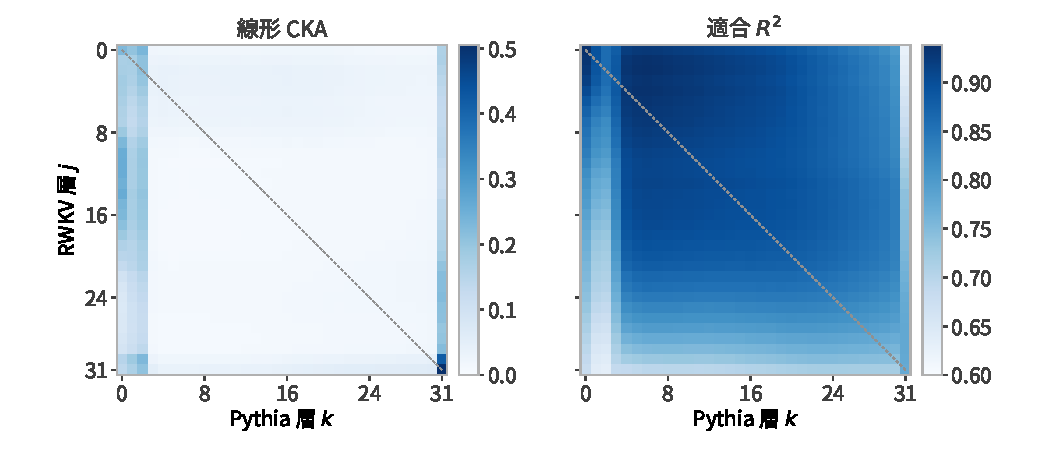
\includegraphics[width=\columnwidth]{fig_layer_cka}
\caption{生残差の全 $32{\times}32$ 層対応（正準表 \texttt{paper\_layer\_correspondence.csv} から生成）。
左：線形 CKA は総じて弱く，高い値は層 $0$ の行・列と最終層の角に集中する――対角（破線）は特別でない。
右：同じ各ペアへ層別の線形写像をあてはめた適合 $R^2$ は $0.62$--$0.94$ とほぼ全ペアで高い。
二つのパネルの色スケールは異なる。}
\label{fig:cka}
\end{figure}整合が\emph{学習可能}であることは確認できるが，
その射程はこの意味でも限定的である（\S\ref{sec:discussion}）。

以降の数値はすべて，同一構成の単一の学習から得たものである。潜在の幅は $z{=}d{=}4096$（圧縮なし），$32$ ブロック
すべてを対応付け，アダプタは $268.5$M パラメータ，$\sigma{=}0.4$，学習率は $10^{-3}$ から plateau 方式で下限 $10^{-5}$
まで下げた。学習信号は Alpaca 学習分割の $2{,}075$ 窓（各 $112$ トークン，独立トークン位置 $\approx\!232$k）から取った残差で，
$32$ 層で $7.44$M ペアを成し，このペア集合を約 $228$ 回反復した。報告値は，保留 $A\!\to\!B$ が最良となる
最深点（$415{,}000$ 反復）のチェックポイントのものである（学習走行と収束の記録は付録~\ref{sec:repro}）。\PtoR{} の系統横断写像は $B\!\to\!A\ 0.590$ で，わずかに
$A\!\to\!B\ 0.559$ を上回る（RNN 側の残差の方が Transformer 潜在から復元しやすい）。両者とも自系統再構成
（$A\!\to\!A\ 0.695$，$B\!\to\!B\ 0.711$）を下回っており，系統横断が整合ではなく復号で律速されることを裏づける。
これらの整合・読み出しがトークンごとの真の対応であって分布の重なりではないことは，負の対照で確かめた：$A$ の行順を保ったまま
$B$ の残差行を単一の乱数置換で入れ替えて再対応させると，$\rho_{\mathrm{ctr}}$ は $0.901\!\to\!0.000$，
$A\!\to\!B$ は $0.561\!\to\!-0.592$，$B\!\to\!A$ は $0.592\!\to\!-0.609$ へ崩壊する
（自系統写像 $A\!\to\!A$，$B\!\to\!B$ は構成上不変）。すなわち両方向の読み出しとも，正しいトークン対応なしには得られない。

\paragraph{共通モードは些末な問題ではない。}潜在のうちトークンごとに変動する成分の割合
$f=\lVert z-\overline{z}\rVert^2/\lVert z\rVert^2$ を導入すると，この落とし穴を定量化できる。要素ごとの係数を持たない
層正規化のもとで，生の相関は
$\rho_{\mathrm{raw}}=(1-f)+f\,\rho_{\mathrm{ctr}}$，すなわち $\text{align}=2f(1-\rho_{\mathrm{ctr}})$ と
分解される。ここで報告する $f$ は $A,B$ それぞれの変動割合の平均であり，この形が等式として成り立つのは両者が等しく，
かつ両者の共通モードが平行な場合である。実測では，学習が進んだ後の評価点でこの関係は $3\!\times\!10^{-4}$ 程度の
精度で成り立つ。ただし学習初期には成り立たず，$0$ 反復目では残差が $6.6\!\times\!10^{-2}$ に達する。等式が語るのは，生の相関が\emph{混合物}だということである
――そのうち $1-f$ の割合は，情報を持たない定数項として無償で与えられている。最深点の $f$ は $0.350$ であるから，
\kw{潜在の持つエネルギーの $65\%$ はトークンに依存しない定数}であり，生の相関はその定数に支配される。実際，中心化した
$\rho_{\mathrm{ctr}}$ が $0.901$ であるのに対し生の相関は $0.965$ を示し，等式はこれを
$(1{-}0.350)+0.350\times0.901=0.965$ と過不足なく再現する。$f$ の解釈上の限界（$f$ が大きくても情報を
担うとは限らない）と，生の相関が改善を捉え損なう学習動態の実例は付録~\ref{sec:common-mode} に示す。

\section{両横断読み出しは自系統再構成に制約される}\label{sec:ladder}
測定した五つの診断値を図~\ref{fig:ladder} に示す。
\[
 \begin{array}{ll}
 \multicolumn{2}{l}{\rho_{\mathrm{ctr}}=0.901,}\\
 \Rsq(B\!\to\!B)=0.711, & \Rsq(A\!\to\!B)=0.559,\\
 \Rsq(A\!\to\!A)=0.695, & \Rsq(B\!\to\!A)=0.590 .
 \end{array}
\]
$\rho_{\mathrm{ctr}}$ は相関係数，後四者は決定係数であり，数値の大小を同じ尺度として比較することはできない。
本節の結論は，$\Rsq$ 同士では全 $32$ 層で
$A\!\to\!B\le B\!\to\!B$ かつ $B\!\to\!A\le A\!\to\!A$ であること，および
\S\ref{sec:goal} の自己符号器対照で復号のみの損失が下流性能にも現れることに基づく。

\begin{figure*}[!t]\centering
\begin{tikzpicture}[
  font=\footnotesize, >={Stealth[length=2mm]},
  diag/.style={draw,rounded corners=2pt,minimum width=35mm,minimum height=15mm,align=center}]
  \node[diag,fill=green!18,minimum height=33mm] (align) {潜在整合\\$\rho_{\mathrm{ctr}}=0.901$};
  \node[diag,fill=orange!20,right=15mm of align,yshift=9mm] (selfb)
    {$B$ 自系統再構成\\$\Rsq(B\!\to\!B)=0.711$};
  \node[diag,fill=red!16,right=21mm of selfb] (crossab)
    {\RtoP{} 横断読み出し\\$\Rsq(A\!\to\!B)=0.559$};
  \node[diag,fill=orange!20,right=15mm of align,yshift=-9mm] (selfa)
    {$A$ 自系統再構成\\$\Rsq(A\!\to\!A)=0.695$};
  \node[diag,fill=red!16,right=21mm of selfa] (crossba)
    {\PtoR{} 横断読み出し\\$\Rsq(B\!\to\!A)=0.590$};
  \draw[->,thick] (align.east)--node[above,font=\scriptsize]{復号} (selfb.west);
  \draw[->,thick] (align.east)--node[below,font=\scriptsize]{復号} (selfa.west);
  \draw[->,thick] (selfb)--node[midway,fill=white,inner sep=1pt,font=\tiny,align=center]
    {入力分布\\のずれ} (crossab);
  \draw[->,thick] (selfa)--node[midway,fill=white,inner sep=1pt,font=\tiny,align=center]
    {入力分布\\のずれ} (crossba);
\end{tikzpicture}
\caption{共有潜在から両方向の読み出しまでの診断値。高い中心化相関と不完全な自己再構成が共存し，
\RtoP{}／\PtoR{} の横断読み出しは，それぞれ同じ復号器を使う \Pythiaself{}／\RWKVself{} 自己再構成を全層で下回る。
相関係数と決定係数は異なる尺度であるため，尺度間の数値差そのものを損失量とは解釈しない。}
\label{fig:ladder}
\end{figure*}
高い潜在相関は，高い再構成精度を自動的には保証しない。\RtoP{} は同一の復号器 $D_B$ を通る \Pythiaself{} と，
\PtoR{} は同一の復号器 $D_A$ を通る \RWKVself{} と比較でき，入力が自系統潜在か他系統潜在かだけが異なる。
両不等式は経験的な観測であって定理ではないが，いずれの方向でも自己再構成の段階ですでに相当の誤差があり，
系統横断だけを改善してもその誤差は残る。

\paragraph{圧縮では説明できないが，上限の要因は未解決である。}$B\!\to\!B$ が低いのは潜在が情報を圧縮する
からにすぎない，という反論があり得る。これは議論ではなく，圧縮そのものを取り除くことで確かめられる。$z{=}d{=}4096$
では合成写像 $D\!\circ\!E$ は恒等写像を表現でき，階数による制約は存在しない。それでも $B\!\to\!B$ は $0.711$ に
留まる。ではノイズ $\sigma$ が定める天井なのか――単純なスカラー近似では $0.711$ を説明できず，何が律速して
いるのかは $\sigma$ を掃引するまで確定できないため，本稿では\emph{未解決}として残す。なお $\sigma$ が別の役割――共通モードへの崩壊の抑止――を担うことは $f$ の軌跡が
支持しており，そこは変わらない：圧縮の除去だけでは問題は解消せず，幅の広い潜在は学習初期に潜在エネルギーの
$98\%$ が定数へ崩壊し，回復は学習の終盤まで緩慢である（$f$ の軌跡は付録~\ref{sec:common-mode}）。これは広い潜在を
用いたときにも残る退化であり，共通モードの補正が些末な問題ではない理由でもある。

\section{アダプタは両横断経路で非線形である}\label{sec:linear}
アダプタは 2 つの線形写像に挟まれたゼロ初期化の残差ブロック 1 個であり，学習は純粋な線形写像から始まる。だがそれは
$0$ 反復目の性質であって，$415{,}000$ 反復後の性質ではない。最深点のアダプタが実際どれだけ線形かを，
\RtoP{}／\PtoR{} とも同じ代表 $5$ 層，同じあてはめ行・保留行で測った。

\emph{アダプタのどれだけが線形か。}アダプタ自身の出力を模倣する最良のアフィン写像が説明する出力分散は，
\RtoP{} で $86.6\%$，\PtoR{} で $88.0\%$ である。したがって\kw{残る $13.4\%$／$12.0\%$ は
いかなるアフィン写像でも表現できない}。第二の行列がゼロ初期化だという事実は初期化を語るのみで，
学習後の写像は両経路で明確に非線形である。

\emph{線形写像だけでどこまで届くか。}比較対象はアダプタを近似したものではなく，層ごとに各経路の標準化した
入力残差から標準化した出力残差への最良のアフィン写像を，リッジ付き最小二乗で別々に\emph{直接}あてはめた対照である
（設定の詳細は付録~\ref{sec:repro}）。代表 $5$ 層 $\{4,10,16,22,28\}$ の保留行で評価すると，
最良直接アフィン写像は \RtoP{} $0.487$，\PtoR{} $0.535$ に達する。対応するアダプタは同じ行で \RtoP{} $0.558$，\PtoR{} $0.576$ であり，
非線形写像の増分は $+0.071$／$+0.041$ である。低容量のアフィン写像でも両経路で相当な
系統横断予測ができるため，\emph{共有表現の主張はこの線形到達性で担保される}。

\emph{別途適合したアフィン対照。}表~\ref{tab:bench} では，\RtoP{} のアダプタを直接アフィン写像へ置き換えると
正答率が $8$--$23$ 点崩れる。一方 \PtoR{} では差が小さく，SciQ @8 ではアフィン対照の方が $3.4$ 点高い。
これは経路差として重要だが，二つの写像は学習目的・データ・正則化が異なるため，非線形性の因果効果とはみなさない。

\emph{交絡を抑えた介入：同一アダプタの MLP 枝を無効化する。}そこで，\kw{同一の学習済みアダプタ}の
残差ブロック（唯一の学習非線形性 $\mathrm{fc}_2(\mathrm{GELU}(\mathrm{fc}_1(\cdot)))$）だけを係数 $\alpha$ で
スケールする（$\alpha{=}1$ 完全，$\alpha{=}0$ は\emph{枝を外した同一写像}）。
表現 $R^2$ の $\alpha=0,.25,.5,.75,1$ 掃引は，\RtoP{} で
$-0.41,-0.75,0.35,0.52,0.56$，\PtoR{} で $-0.30,-0.66,0.36,0.53,0.58$ となる。
両経路で枝を外すと負の $R^2$ まで崩れ，しかも非単調である。二つの線形層は残差ブロックと協調して
学習されており，\kw{この学習済みアダプタでは，非線形枝は\RtoP{}だけでなく\PtoR{}の読み出しにも除去不能}である。
これは学習済み写像の性質であって，本課題が線形写像で原理的に解けないことを意味しない（同目的で学習した
線形アダプタとの比較は行っていない）。多肢選択でも同じ $\alpha=0/1$ を
同一問題上でペア化して評価する。

\begin{table}[!htbp]\centering\scriptsize
\caption{同一アダプタの非線形枝を無効化したときの長さ正規化正答率（\%）。
各セルは $\alpha:1\!\to\!0$（完全な学習済み写像 $\to$ 同じ写像から枝のみ除去）を表す。
ARC-Easy $2376$，SciQ $1000$，当て推量 $25\%$。}\label{tab:mlp-intervention}
\setlength{\tabcolsep}{4.2pt}
\resizebox{\columnwidth}{!}{%
\begin{tabular}{rcccc}\toprule
& \multicolumn{2}{c}{ARC-Easy} & \multicolumn{2}{c}{SciQ}\\
\cmidrule(lr){2-3}\cmidrule(lr){4-5}
$L$ & \RtoP{} & \PtoR{} & \RtoP{} & \PtoR{}\\\midrule
4  & $59.6\!\to\!31.9$ & $62.2\!\to\!31.8$ & $70.9\!\to\!31.3$ & $69.2\!\to\!32.6$\\
8  & $59.0\!\to\!29.9$ & $57.3\!\to\!35.5$ & $67.7\!\to\!31.4$ & $64.6\!\to\!37.0$\\
16 & $48.6\!\to\!28.5$ & $57.5\!\to\!43.7$ & $54.5\!\to\!31.7$ & $68.0\!\to\!47.3$\\
24 & $47.0\!\to\!34.8$ & $59.6\!\to\!48.4$ & $51.1\!\to\!40.0$ & $69.9\!\to\!49.1$\\\bottomrule
\end{tabular}}
\end{table}

表~\ref{tab:mlp-intervention} の枝効果は \RtoP{} で $+11.1$--$+39.6$ 点，\PtoR{} で
$+11.2$--$+36.6$ 点であり，$16$ 比較すべてで同一問題上の McNemar 正確検定
$p<2{\times}10^{-9}$ となる。したがって，非線形枝の必要性は一方の経路から推測したものではなく，
\RtoP{}／\PtoR{} の両方の表現と下流精度で直接確認される。

\section{構文的に妥当な生成は得られるが事実性は劣化する}\label{sec:chimera}
ここで実際に $7$B で両横断経路を合成する。切替層 $L$ では，前段親をブロック $0$ から $L$ まで走らせ
（合計 $L{+}1$ ブロック），その残差を \S\ref{sec:method} の境界式で\emph{一度}だけ他方の空間へ翻訳し，
後段親のブロック $L{+}1$ 以降と言語モデルヘッドを走らせる――ブロックごとの往復ではない。
したがって \RtoPL{16} は RWKV $17$ ブロックと Pythia $15$ ブロック，\PtoRL{16} はその反対で，いずれも厳密な半分ではない。

\begin{figure*}[!t]\centering
\begin{tikzpicture}[
  font=\scriptsize, >={Stealth[length=2mm]},
  a/.style={draw,rounded corners=1pt,minimum height=7mm,minimum width=6mm,fill=blue!12},
  b/.style={draw,rounded corners=1pt,minimum height=7mm,minimum width=6mm,fill=orange!14},
  hd/.style={draw,rounded corners=1pt,minimum height=7mm,minimum width=8mm,fill=gray!12},
  tr/.style={draw,rounded corners=2pt,minimum height=10mm,minimum width=13mm,fill=green!14,align=center}]
% \RtoP{} row
\node[font=\bfseries] (labAB) {\RtoP{}};
\node[right=3mm of labAB] (idsAB) {ids};
\node[a,right=3mm of idsAB] (a0) {$A_0$};
\node[right=1.5mm of a0] (ad) {$\cdots$};
\node[a,right=1.5mm of ad] (aL) {$A_L$};
\node[tr,right=3mm of aL] (tab) {$E_A\!\to z$\\$\to D_B$};
\node[b,right=3mm of tab] (bN) {$B_{L+1}$};
\node[right=1.5mm of bN] (bd) {$\cdots$};
\node[b,right=1.5mm of bd] (b31) {$B_{31}$};
\node[hd,right=2.5mm of b31] (hb) {$B$ head};
\node[right=2.5mm of hb] (outAB) {logits};
\draw[->] (idsAB)--(a0);
\foreach \x/\y in {a0/ad,ad/aL,aL/tab,tab/bN,bN/bd,bd/b31,b31/hb,hb/outAB} \draw[->] (\x)--(\y);
% \PtoR{} row, aligned by role with \RtoP{}
\node[font=\bfseries,below=12mm of labAB] (labBA) {\PtoR{}};
\node[right=3mm of labBA] (idsBA) {ids};
\node[b,right=3mm of idsBA] (bb0) {$B_0$};
\node[right=1.5mm of bb0] (bbd) {$\cdots$};
\node[b,right=1.5mm of bbd] (bbL) {$B_L$};
\node[tr,right=3mm of bbL] (tba) {$E_B\!\to z$\\$\to D_A$};
\node[a,right=3mm of tba] (aaN) {$A_{L+1}$};
\node[right=1.5mm of aaN] (aad) {$\cdots$};
\node[a,right=1.5mm of aad] (aa31) {$A_{31}$};
\node[hd,right=2.5mm of aa31] (ha) {$A$ head};
\node[right=2.5mm of ha] (outBA) {logits};
\draw[->] (idsBA)--(bb0);
\foreach \x/\y in {bb0/bbd,bbd/bbL,bbL/tba,tba/aaN,aaN/aad,aad/aa31,aa31/ha,ha/outBA} \draw[->] (\x)--(\y);
\node[font=\tiny,above=3mm of tab,align=center] {
  \textcolor{blue!55!black}{$A=$ RWKV（KV 不要）}\qquad
  \textcolor{orange!65!black}{$B=$ Pythia（KV 要）}
};
\end{tikzpicture}
\caption{\RtoP{}／\PtoR{} キメラの対称な構成。図中左側の親をブロック $L$ まで実行し，残差を一度だけ翻訳して，
右側の親のブロック $L{+}1$ 以降とヘッドへ渡す。青は RWKV-Raven，橙は Tulu-Pythia。
したがって Transformer 層数は \RtoP{} で $31{-}L$，\PtoR{} で $L{+}1$ となる。}
\label{fig:chimera}
\end{figure*}

最深点の同一アダプタを \RtoP{}／\PtoR{} とも $L{=}4$ に挿入し，同じ四つの英語プロンプトを
温度 $0$，最大 $40$ 新規トークンで貪欲復号した。$L{=}4$ は，二課題平均が各横断方向の四境界中で最大であり，
SciQ の KV--精度平面でも両方向が非支配集合に入る共通境界である（図~\ref{fig:tradeoff}）。
ただしこれは同じ報告タスクを見た後の代表点選択であり，独立な生成用選択基準ではない。
本比較は網羅的な生成ベンチマークではないが，少なくとも一方の横断読み出しから他方の生成を推測せず，
両方の end-to-end 配線を同条件で観察する。

\begin{table*}[!t]\centering\footnotesize
\setlength{\tabcolsep}{4pt}
\caption{最深点アダプタの \RtoP{}／\PtoR{} による再生成結果（ともに $L{=}4$）と，両親 pure Pythia／pure RWKV の
同一プロンプト出力。英語原文をそのまま入力し，temperature $0$ の argmax，最大 $40$ 新規トークン，EOS のみ早期終了とした。
各キメラは後段親の隣に置く。長い反復は要約し，逐語出力は
\texttt{paper\_cross\_family\_generation\_samples.csv} に収録する。
四つのプロンプトに限る定性的比較であり，生成品質の定量評価ではない。}\label{tab:generation}
\begin{tabular}{|p{0.145\linewidth}|p{0.18\linewidth}|p{0.19\linewidth}|p{0.16\linewidth}|p{0.19\linewidth}|}\hline
Prompt (verbatim) & pure Pythia &
\RtoP{}\par{\scriptsize 横断読み出し $R^2{=}0.559$} &
pure RWKV &
\PtoR{}\par{\scriptsize 横断読み出し $R^2{=}0.590$}\\\hline
{\ttfamily \#\#\# Instruction:\par
What is the capital of France?\par\smallskip
\#\#\# Response:} &
``The capital of France is Paris.'' & \textbf{``The capital of France is Paris.''} \checkmark &
``Paris.'' & \textbf{``Paris.''} \checkmark\\\hline
{\ttfamily The three primary colors are} &
``red, yellow, and blue. These colors are often used in combination to create a wide variety of colors.'' & \textbf{``red, yellow, and blue.''} \checkmark &
``red, blue, and yellow.'' と正答後，赤の反対色（緑）を問う Q\&A へ逸脱 &
``red, blue, and yellow.'' と正答後，Bob/Alice の緑についての対話へ逸脱\\\hline
{\ttfamily Question: Water is made of hydrogen and\par Answer:} &
``Hydrogen is made of hydrogen and oxygen.'' &
``Hydrogen.'' \textbf{（誤り）} &
``hydrogen.'' \textbf{（誤り）} & ``hydrogen.'' \textbf{（誤り）}\\\hline
{\ttfamily \#\#\# Instruction:\par
Explain what a black hole is in one sentence.\par\smallskip
\#\#\# Response:} &
``A black hole is a region of spacetime where gravity is so strong that nothing, not even light, can escape its pull.'' &
``A black hole is a region in space where gravity is so strong that nothing, not even light, can escape its pull.'' \checkmark &
``A black hole is a region of space where the gravitational pull is so strong that nothing, not even light, can escape.'' &
``A black hole is a type of celestial object that is formed when a star collapses and collapses into a black hole.''
\emph{（循環的）}\\\hline
\end{tabular}
\end{table*}

これらの例から二点が観察できる。第一に，\kw{\RtoP{}／\PtoR{} とも構文的にもっともらしい出力を生成できる}。両方がフランスの首都へ正答し，
三原色も正しく開始する。\RtoP{} はブラックホールにも一文で正答するため，いずれか一方向の表現指標だけから
動作を推測した結果ではない。第二に，\kw{流暢さが保たれても内容や指示形式を失い得る}。両方向とも水の補完を
``hydrogen'' と誤り，\PtoR{} は三原色への正答後に対話形式へ逸脱し，ブラックホールを循環的に説明する。
したがって $0.559/0.590$ の横断読み出しでも事実性は十分でない。より忠実なキメラには両横断読み出しと
自系統再構成の改善が必要である。

\section{親モデルとの機能・推論メモリ比較}\label{sec:goal}
NinaXander の実用上の価値を評価するには，内部表現の指標だけでなく，凍結した両親との機能比較が必要である。
ここでは，(i) 強い親モデルに対してどこまで性能を保てるか，(ii) 弱い親または同じ KV 容量の Transformer を
上回るか，(iii) その代わりにどの程度のメモリを削減できるかを測る。

この比較は，各選択肢の対数尤度を求めて最大のものを選ぶ多肢選択形式で行う。生成も文字列の照合も主観的な判定も
介在しないため，結果は一意に定まる。用いたのは\kw{全評価集合}（ARC-Easy test $2376$，SciQ test $1000$），最深点
（$415{,}000$ 反復）の $z{=}4096$ のアダプタ，そして四つの切替位置である。同一問題集合上の構成間比較はペア化データなので，
差はセルごとの独立な二項 SE ではなく\kw{ペア化検定}（McNemar の正確検定と対応 bootstrap）で評価する。選択肢は長さが
異なり総和／長さ正規化で順位が食い違い得るので両方を構造化データに保存し，本文は長さ正規化を報告・検定に用いる。
また SciQ は付属の support 文を与えない closed-book 形式（Question／Answer のみ）で評価するため，本稿の SciQ 値は
support を与える標準プロトコルの公表値と直接比較できない。

\begin{table}[!htbp]\centering\scriptsize
\caption{\RtoP{}／\PtoR{} の学習済みアダプタと，各経路の入力・出力残差へ別々に適合した最良アフィン対照による
長さ正規化多肢選択正答率（\%，ARC-Easy $2376$，SciQ $1000$，当て推量 $25$）。
各値は同じ問題，同じ切替層，同じ後段実行を用いる。}\label{tab:bench}
\setlength{\tabcolsep}{2.8pt}
\resizebox{\columnwidth}{!}{%
\begin{tabular}{rcccccccc}\toprule
& \multicolumn{4}{c}{ARC-Easy} & \multicolumn{4}{c}{SciQ}\\
\cmidrule(lr){2-5}\cmidrule(lr){6-9}
& \multicolumn{2}{c}{\RtoP{}} & \multicolumn{2}{c}{\PtoR{}}
& \multicolumn{2}{c}{\RtoP{}} & \multicolumn{2}{c}{\PtoR{}}\\
$L$ & adapter & affine & adapter & affine
& adapter & affine & adapter & affine\\\midrule
4  & 59.6 & 41.9 & 62.2 & 60.2 & 70.9 & 47.5 & 69.2 & 69.6\\
8  & 59.0 & 43.1 & 57.3 & 56.0 & 67.7 & 49.1 & 64.6 & 68.0\\
16 & 48.6 & 34.8 & 57.5 & 57.5 & 54.5 & 35.9 & 68.0 & 69.6\\
24 & 47.0 & 39.4 & 59.6 & 59.2 & 51.1 & 42.7 & 69.9 & 68.2\\\bottomrule
\end{tabular}}
\end{table}

\begin{table}[!htbp]\centering\scriptsize
\caption{4 経路の長さ正規化正答率（\%）。
\RWKVself{}／\Pythiaself{} は自系統再構成対照，\RtoP{}／\PtoR{} は系統横断キメラ。
同じ問題・切替層の二つの横断経路差はペア化して検定した。}
\label{tab:direction}
\setlength{\tabcolsep}{3.2pt}
\resizebox{\columnwidth}{!}{%
\begin{tabular}{rcccccccc}\toprule
& \multicolumn{2}{c}{\RWKVself{}} & \multicolumn{2}{c}{\RtoP{}}
& \multicolumn{2}{c}{\Pythiaself{}} & \multicolumn{2}{c}{\PtoR{}}\\
$L$ & ARC & SciQ & ARC & SciQ & ARC & SciQ & ARC & SciQ\\\midrule
4  & 62.8 & 68.5 & 59.6 & 70.9 & 62.2 & \textbf{74.8} & \textbf{62.2} & 69.2\\
8  & 59.8 & 66.7 & 59.0 & 67.7 & 62.7 & \textbf{74.8} & 57.3 & 64.6\\
16 & 54.8 & 59.8 & 48.6 & 54.5 & 57.4 & \textbf{71.1} & \textbf{57.5} & 68.0\\
24 & 52.2 & 57.9 & 47.0 & 51.1 & 59.4 & \textbf{70.1} & \textbf{59.6} & 69.9\\\bottomrule
\end{tabular}}
\end{table}

四経路の同時比較から六つのことが読み取れる。\emph{(a)} \kw{$7$B の半分が外来であっても，\RtoP{}／\PtoR{} とも実際に問いへ
答えられる}。全横断構成が当て推量を大きく上回り，SciQ では \RtoP{} $70.9\%$，\PtoR{} $69.9\%$ に達する。
\emph{(b)} \kw{深さ効果は経路依存}である。\RtoP{} は $L=4\to24$ で SciQ
$70.9\to67.7\to54.5\to51.1$，ARC-Easy $59.6\to59.0\to48.6\to47.0$ と単調に下がるが，
\PtoR{} は SciQ $69.2\to64.6\to68.0\to69.9$，ARC-Easy $62.2\to57.3\to57.5\to59.6$ と非単調である。
局所読み出しは同じ四層で \RtoP{} $0.570/0.555/0.575/0.567$，\PtoR{} $0.552/0.517/0.604/0.608$ であり，
層番号や一つの局所 $R^2$ だけから end-to-end の順位は決まらない。
\emph{(c)} \kw{強いほうの親はどちらの経路でも超えられない}。全 $8$ 横断構成が両タスクで Tulu-Pythia を下回り，
各同一問題の McNemar 検定でも有意である。
\emph{(d)} \kw{RWKV に対する差も経路・課題依存}である。\RtoPL{4} は SciQ で RWKV を $+3.9$ 点
（$p{=}0.018$）上回る一方，ARC-Easy では $-2.2$ 点（$p{=}0.042$）である。ただし総和スコアではこの優位は消える
（\RtoPL{4} は SciQ $-2.7$ 点，\PtoRL{4} は ARC $-4.6$ 点／SciQ $-5.7$ 点）――弱い親に対する優劣の判定は
長さ正規化の選択に依存する。\PtoR{} はいずれの境界も RWKV を
有意に上回らず，\PtoRL{4} は ARC $+0.4$ 点（$p{=}0.66$），SciQ $+2.2$ 点（$p{=}0.14$）で統計的に同等である。
\emph{(e)} \kw{別途適合したアフィン対照の差も経路依存}である。\RtoP{} ではアダプタが全セルで $8$--$23$ 点高いが，
\PtoR{} では差が小さく，SciQ @8 ではアフィンが $3.4$ 点高い。この比較は写像自体が異なるため記述的であり，
同一アダプタの非線形枝を操作する因果的な比較は \S\ref{sec:linear} の $\alpha$ 介入で両経路について行う。
\emph{(f)} \kw{自系統対照との差は翻訳誤差だけではない}。B 後段では純 Pythia，\Pythiaself{}，\RtoP{} の順に下がり，
\Pythiaself{}--\RtoP{} 差は SciQ $4$--$19$ 点，ARC $3$--$12$ 点である。一方 A 後段では \PtoR{} が \RWKVself{} を深い境界で逆に上回り，
$L=16/24$ の差は ARC $+2.7/+7.4$ 点，SciQ $+8.2/+12.0$ 点となる。
したがって自系統対照は復号段を切り分けるが，横断との差には前段親の能力と翻訳のずれがともに入り，
普遍的な「翻訳コスト」にはならない。

\paragraph{\RtoP{} と \PtoR{} では深さ依存が異なる.}表~\ref{tab:direction} のとおり，\PtoR{} は $L{=}16,24$ で同じ層の \RtoP{} を
ARC で $+8.9/+12.6$ 点，SciQ で $+13.5/+18.8$ 点上回る（同一問題の McNemar 検定，すべて
$p<3{\times}10^{-15}$）。一方，$L{=}4$ は ARC で $+2.6$ 点（$p{=}0.015$）だが SciQ で $-1.7$ 点
（$p{=}0.28$）であり，浅い境界では経路差は一様でない。したがって，\RtoP{} で見えた単調な深さ効果を「同じ番号の層を
つなぐ難しさ」と一般化できない。どの \PtoR{} 構成も Pythia を有意に下回る。また RWKV に対して有意に優る \PtoR{} 構成はなく，
\PtoRL{4} は ARC $62.2$ 対 $61.8$（$p{=}0.66$），SciQ $69.2$ 対 $67.0$（$p{=}0.14$）で同等である。

\PtoR{} の最良アフィン写像は，各切替層でアダプタと別に適合した対照である。ARC @4 ではアダプタが $+2.0$ 点
（$p{=}0.005$）だが，他の多くは差がなく，SciQ @8 では逆にアフィンが $+3.4$ 点（$p{=}0.003$）である。
この写像間比較とは別に，同一アダプタの非線形枝を $\alpha=0$ とする介入を \RtoP{}／\PtoR{} の同じ四層・同じ問題で実行し，
因果的な非線形枝の寄与はそのペア化結果から評価する。$A\!\to\!A$ 自己符号器との比較も，
RWKV 前段を Pythia 前段と横断翻訳へ同時に置き換えるため，翻訳誤差だけを分離しない。

\paragraph{配布既定値は「最良実測」であって外部検証ではない.}両タスクの正答率を単純平均すると，\PtoRL{4} は
$65.70\%$，\RtoPL{4} は $65.25\%$ で差はわずか $0.45$ 点である。完全版は経路を明示して分割し，
\nolinkurl{ninaxander-tulu69-to-raven7b-best} は \PtoRL{4}，
\nolinkurl{ninaxander-raven7b-to-tulu69-best} は \RtoPL{4} を各経路内の既定値とする。
runtime はパッケージ名と反対の経路への切替を拒否する一方，境界比較用の $L{=}8,16,24$ plan は保持する。
いずれも同じ二つの報告テスト集合上で各経路の四境界から選んだ\emph{事後的}順位であり，独立な
deployment-selection 分割を持たない。したがって，未知の実行経路一般への改善や汎化性能の優越を主張する根拠には用いない。

\paragraph{合成によるメモリ上の効果：Transformer 層とともに KV キャッシュが消える。}性能と推論メモリは同時に評価する必要がある。
二つの系統は推論時の費用が同じではないからである。Transformer の層はトークンごとに key/value をキャッシュする
が，RNN 層が持つのは\kw{系列長に対して $O(1)$} の再帰状態である。\RtoP{} は Transformer を $31{-}L$ 層，
\PtoR{} は $L{+}1$ 層だけ保持する。Tulu-Pythia のキャッシュは仮定でなく\emph{実測}した：
層あたり $16.0$ KiB/token，$32$ 層で $512$ KiB/token（$2Ld\cdot2$\,bytes と厳密に一致）。

\begin{table*}[!t]\centering\footnotesize
\caption{\RtoP{}／\PtoR{} 両経路の正答率と推論メモリ。KV は実測値；RWKV 再帰状態は文脈長に対して定数である。}\label{tab:kv}
\begin{tabular}{lccccc}\toprule
構成 & Transformer 層 & KV / token & KV @ $4$k 文脈 & 削減 & ARC / SciQ\\\midrule
pure Tulu-Pythia & 32 & $512$ KiB & $2.00$ GiB & --- & 65.3 / 81.0\\
\RtoPL{4}  & 27 & $432$ KiB & $1.69$ GiB & $15.6\%$ & 59.6 / 70.9\\
\RtoPL{8}  & 23 & $368$ KiB & $1.44$ GiB & $28.1\%$ & 59.0 / 67.7\\
\RtoPL{16} & 15 & $240$ KiB & $0.94$ GiB & $53.1\%$ & 48.6 / 54.5\\
\RtoPL{24} &  7 & $112$ KiB & $0.44$ GiB & $78.1\%$ & 47.0 / 51.1\\
\PtoRL{24} & 25 & $400$ KiB & $1.56$ GiB & $21.9\%$ & 59.6 / 69.9\\
\PtoRL{16} & 17 & $272$ KiB & $1.06$ GiB & $46.9\%$ & 57.5 / 68.0\\
\PtoRL{8}  &  9 & $144$ KiB & $0.56$ GiB & $71.9\%$ & 57.3 / 64.6\\
\textbf{\PtoRL{4}} & \textbf{5} & \textbf{$80$ KiB} & \textbf{$0.31$ GiB} &
\textbf{$84.4\%$} & \textbf{62.2 / 69.2}\\
pure RWKV-Raven & 0 & $0$ & $0$ & $100\%$ & 61.8 / 67.0\\\bottomrule
\end{tabular}
\end{table*}

\RtoP{}／\PtoR{} を含めると，\PtoRL{4} は \RtoPL{4} より Transformer 層を $27\to5$ へ減らしながら，二タスク平均を
$65.25\%\to65.70\%$ とほぼ保つ。置き換える RWKV の再帰状態は層あたり $40$ KiB（$5$ 状態ベクトル ${\times}\,4096$ 次元 ${\times}$ fp16 からの算出値）で，構成上文脈長に依存しない。
ただし純 RWKV は KV がゼロであり，順位はタスクに依存するため，図~\ref{fig:tradeoff} は SciQ に限った
メモリ--精度フロンティアとして示す。

\begin{figure}[!htbp]\centering
\begin{tikzpicture}[font=\scriptsize,>={Stealth[length=2mm]}]
  \def\xs{0.62}
  \def\ys{0.15}
  \draw[->] (0,0) -- (68mm,0);
  \draw[->] (0,0) -- (0,5.6) node[above left,font=\scriptsize,align=left] {SciQ\\正答率};
  \node[font=\scriptsize] at (34mm,-8mm) {KV キャッシュ削減率（\%）};
  \foreach \x in {0,20,40,60,80,100} \draw (\x*\xs/10,-1pt) node[below,font=\tiny]{\x} -- (\x*\xs/10,2pt);
  \foreach \y in {55,65,75} \draw (-1pt,{(\y-50)*\ys}) node[left,font=\tiny]{\y} -- (2pt,{(\y-50)*\ys});
  \coordinate (pP) at (0,{(81.0-50)*\ys});
  \coordinate (ab4) at ({15.625*\xs/10},{(70.9-50)*\ys});
  \coordinate (ab8) at ({28.125*\xs/10},{(67.7-50)*\ys});
  \coordinate (ab16) at ({53.125*\xs/10},{(54.5-50)*\ys});
  \coordinate (ab24) at ({78.125*\xs/10},{(51.1-50)*\ys});
  \coordinate (ba4) at ({84.375*\xs/10},{(69.2-50)*\ys});
  \coordinate (ba8) at ({71.875*\xs/10},{(64.6-50)*\ys});
  \coordinate (ba16) at ({46.875*\xs/10},{(68.0-50)*\ys});
  \coordinate (ba24) at ({21.875*\xs/10},{(69.9-50)*\ys});
  \coordinate (rw) at ({100*\xs/10},{(67.0-50)*\ys});
  \draw[green!50!black,thick] (pP)--(ab4)--(ba24)--(ba4)--(rw);
  \fill[black] (pP) circle (1.8pt);
  \foreach \p in {ab4,ab8,ab16,ab24} \fill[blue!70!black] (\p) circle (1.7pt);
  \foreach \p in {ba4,ba8,ba16,ba24}
    \node[fill=orange!80!black,rectangle,minimum size=3.4pt,inner sep=0pt] at (\p) {};
  \fill[red!70!black] (rw) circle (1.8pt);
  \node[above right=-1pt and 1pt of pP,font=\tiny] {pure Pythia};
  \node[above left=-1pt and 1pt of ab4,font=\tiny,text=blue!60!black] {$L=4$};
  \node[below=1pt of ab8,font=\tiny,text=blue!60!black] {$L=8$};
  \node[below=1pt of ab16,font=\tiny,text=blue!60!black] {$L=16$};
  \node[below=1pt of ab24,font=\tiny,text=blue!60!black] {$L=24$};
  \node[above left=-1pt and 1pt of ba4,font=\tiny,text=orange!70!black] {$L=4$};
  \node[below=1pt of ba8,font=\tiny,text=orange!70!black] {$L=8$};
  \node[above=1pt of ba16,font=\tiny,text=orange!70!black] {$L=16$};
  \node[below right=-1pt and 1pt of ba24,font=\tiny,text=orange!70!black] {$L=24$};
  \node[above left=-1pt and 1pt of rw,font=\tiny,text=red!60!black] {pure RWKV};
  \node[align=left,font=\tiny,fill=white,rounded corners=1pt,inner sep=2pt] at (42mm,5.25)
    {\textcolor{blue!70!black}{$\bullet$} \RtoP{}（RWKV 前段）\quad
     \textcolor{orange!80!black}{$\blacksquare$} \PtoR{}（Pythia 前段）\\
     \textcolor{green!50!black}{\rule[0.3ex]{4mm}{0.8pt}} SciQ 非支配フロンティア};
\end{tikzpicture}
\caption{\RtoP{}／\PtoR{} の SciQ 正答率と実測 KV 削減率。両経路を含む非支配点は
pure Pythia $\to$ \RtoPL{4} $\to$ \PtoRL{24} $\to$ \PtoRL{4} $\to$ pure RWKV（緑）となる。
これは SciQ 一課題上の事後的フロンティアであり，
経路一般の優越や未知課題への汎化を意味しない。}
\label{fig:tradeoff}
\end{figure}
Pythia 前段の経路を加えると，高削減点 \PtoRL{4} が得られる。この点は RWKV 前段の経路だけでは現れない。
一方，pure RWKV は依然 KV ゼロであり，
\PtoRL{4} が RWKV を有意に上回るわけでもない。したがって利点は，凍結親の間に\emph{追加の交換点}を作れることであって，
新しい構成が親を一律に支配することではない。

\paragraph{等 KV の Transformer 基準と，未使用ブロックを除いた推論実装.}Transformer 親側の効率化との比較を実測した。
\RtoP{} では同じ $31{-}L$ Transformer ブロックを持つ Pythia early exit と比べ，@16/@24 のキメラが
ARC $+11.2/+18.5$，SciQ $+12.8/+18.7$ 点上回る一方，@4 は同点である。\PtoR{} では，同じ $L{+}1=5/9/17/25$
ブロックの early exit に対し，キメラは ARC $+35.4/+27.6/+16.9/+2.1$，SciQ
$+38.7/+31.6/+17.9/+0.5$ 点である。最初の三境界は有意，25 ブロックでは同点（ARC $p{=}0.069$，
SciQ $p{=}0.80$）であり，Pythia 前段がごく浅いとき RWKV 後段が実際の機能を補う。

未使用ブロックを物理的に除く経路も \RtoP{}／\PtoR{} に実装した。\PtoR{} では Pythia 前段，RWKV 後段，両者をつないだ完全経路を
それぞれ未剪定参照と比較し，全 $4$ 境界で $\mathrm{rel}{=}0$ である。常駐重みは \RtoP{} $13.93$--$14.55$\,GiB，
\PtoR{} $13.49$--$14.11$\,GiB（既定の \PtoRL{4} は $14.11$\,GiB）で，完全な両親 $27$\,GiB のほぼ半分となる。ただし対応する
Pythia early exit は \PtoR{} で $2.64$--$10.14$\,GiB とさらに軽い。さらに参照 runtime は最適化した serving engine ではない：
HF RWKV を系列方向に逐次実行し，cacheless decode では prefix を毎回再計算する。\PtoRL{4} の文脈 $2048$ prefill は
剪定後も $22.6$ 秒（pure Pythia $0.378$ 秒），未剪定の cacheless decode は $0.148$ token/s
（Pythia $9.49$ token/s）である。これらは現在の正しさ優先実装の値であり，アーキテクチャ固有の速度限界ではない。
KV 量子化・sliding-window との比較も行っていない。

親モデルとの比較結果は限定付きである：\kw{機能は保つが，正答率の一律な向上ではない}。\RtoP{}／\PtoR{} とも強い Pythia を
有意に下回る。\RtoP{} は RWKV を SciQ でのみ上回り，\PtoR{} はどの境界も RWKV を有意に上回らない。得られた主な利点は，
\PtoRL{4} で Pythia の正答率の一部を保ちながら Transformer KV を $84.4\%$ 除けることである。

\paragraph{翻訳は領域特異的である。}以上の正答率は，指示形式に近い短い設問で測ったものである。KV キャッシュの
節約が意味を持つのは長い文脈であり，そこでキメラが\emph{開放テキストの言語モデリング}をどれだけ保つかは別に測る必要が
ある。文脈 $512$ の \RtoPL{4} は Alpaca で perplexity $6.40$，WikiText-103 で $93.87$ である。\PtoRL{4} は
$3.85/45.00$ と両領域で改善するが，WikiText はなお親の $11.33/16.22$ から大きく離れる。文脈を $2048$ へ伸ばすと
\PtoRL{4} は Alpaca $3.50$，WikiText $34.78$ となり，崩壊せずむしろ改善する。したがって主因は文脈長でなく
\emph{領域シフト}である。\PtoR{} はシフトを緩和するが，WikiText $34.78$ は良い方の親 RWKV $8.27$ の $4.2$ 倍であり，
問題を解消しない。

各切替層の線形対照は，Alpaca と WikiText の各先頭 $40{,}000$ token で\emph{別々に再推定}し，それぞれの非重複 suffix で
評価した supervised affine oracle である。WikiText の値は Alpaca で推定した写像の領域外汎化ではなく，学習済み
アダプタとも目的・データが異なる。ゆえにアフィンとの優劣から「非線形部分だけが領域に過適合した」とは結論しない。
領域特異性の根拠は，同じ学習済みアダプタが Alpaca と WikiText で親に対する相対性能を大きく変えることにある。

\begin{figure}[!htbp]\centering
\resizebox{\columnwidth}{!}{%
\begin{tikzpicture}[font=\scriptsize]
  % log-scale perplexity bars, in-domain (Alpaca) vs out-of-domain (WikiText), ctx 512. 1 decade = 1.2cm.
  \def\Y#1{ {12*ln(#1)/ln(10)/10} }
  \draw[->] (0,0) -- (0,3.7) node[above,font=\scriptsize] {パープレキシティ（対数）};
  \foreach \v in {3,10,30,100,300} \draw[gray!30] (0,\Y{\v}) node[left,font=\tiny,black]{\v} -- (84mm,\Y{\v});
  \draw[thick] (0,0) -- (84mm,0);   % x baseline
  \def\grp#1#2#3#4{  % xcenter(mm), label, alpaca_ppl, wiki_ppl
    \fill[teal!60] (#1mm-4.2mm,0) rectangle (#1mm-0.4mm,\Y{#3});
    \fill[red!40]  (#1mm+0.4mm,0) rectangle (#1mm+4.2mm,\Y{#4});
    \node[font=\tiny,below=1pt] at (#1mm,0) {#2};
  }
  \grp{11}{RWKV}{3.42}{11.33}
  \grp{33}{Pythia}{5.19}{16.22}
  \grp{55}{\shortstack{RWKV$\to$\\Pythia\\$L=4$}}{6.40}{93.87}
  \grp{77}{\shortstack{Pythia$\to$\\RWKV\\$L=4$}}{3.85}{45.00}
  % legend in the empty top-left (above the short parent bars)
  \fill[teal!60] (3mm,3.25) rectangle (7mm,3.45);
  \node[font=\tiny,anchor=west] at (7mm,3.35) {領域内 Alpaca};
  \fill[red!40]  (27mm,3.25) rectangle (31mm,3.45);
  \node[font=\tiny,anchor=west] at (31mm,3.35) {領域外 WikiText};
\end{tikzpicture}}
\caption{領域シフト（文脈 $512$，対数軸）。\PtoR{} は \RtoPL{4} の
WikiText perplexity を $93.87\to45.00$ に改善するが，両親 $11.33/16.22$ には届かない。同じアダプタが
Alpaca では親の近傍にあるため，長さでなく領域が主要な差である。}
\label{fig:domain}
\end{figure}

\section{関連研究}\label{sec:related}
\paragraph{モデル・スティッチング.}凍結した $2$ モデルの層を学習可能な接合層でつなぐ手法は，表現の\emph{等価性}を測る
ために Lenc と Vedaldi~\cite{10.1007/s11263-018-1098-y} が導入し，Bansal ら~\cite{3540261.3540279} が表現比較のプローブとして再訪した。
いずれも\emph{同一アーキテクチャ・同一課題}での接合であり，本研究は異なる\emph{系統}（RNN$\leftrightarrow$Transformer）を
各層で $1$ 度だけ翻訳する共有潜在で接合する点で異なる。
\paragraph{凍結 LLM の合成.}近年は凍結した LLM どうしを学習可能な接続で合成する研究が続いている。
StitchLLM~\cite{hu-etal-2025-stitchllm} は規模の異なる Transformer のブロックを stitching 層で接いで serving 時に
経路を選び，BTS~\cite{zhang-etal-2025-bts} は同一シードから分岐した専門家群を stitch 層でシードへ再結合する。
CALM~\cite{bansal2024llm} は凍結した 2 つの Transformer の中間表現を cross-attention で融合し，
Manticore~\cite{roberts2025pretrained} は Transformer と Mamba のブロックを射影で接いだハイブリッドを
\emph{end-to-end に微調整}する。
ただし，これらは両側が Transformer（BTS は同一シード）であるか，合成体を微調整する（Manticore）。我々の知る限り，凍結した純 RNN と凍結 Transformer の残差を\emph{双方向}に翻訳して
単一境界で合成し，KV 削減量まで実測した研究はない。
\paragraph{表現類似度.}CKA~\cite{pmlr-v97-kornblith19a} や (SV/PW)CCA~\cite{3295222.3295356,3327345.3327475} はネットワーク間の表現
類似度を測る標準的な道具である。本研究はこれらを補助指標として用いつつ（\S\ref{sec:space} の全層対応），主眼を
\emph{再構成を介した機能的な}接合に置く。
\paragraph{モデルマージ・知識統合.}重み空間でモデルを統合する model soups~\cite{pmlr-v162-wortsman22a}，TIES~\cite{3666122.3666432}，進化的マージ~\cite{Akiba2025} は，
\emph{同一または互換な}重みを前提とする。出力分布を融合する FuseLLM~\cite{wan2024knowledge} は重みの互換を要しないが，
語彙間のトークン整列と対象モデルの継続学習を必要とする。本研究は重みを
一切マージせず\emph{活性化空間}を翻訳して凍結ブロックを組み替える点で相補的である。
\paragraph{対象モデル.}RWKV~\cite{peng-etal-2023-rwkv} は softmax 自己注意を持たず推論時に純粋な再帰として動作するアーキテクチャであり，本研究ではその第 4 世代の指示追従版 RWKV-4-Raven-7B を用いる。Pythia~\cite{3618408.3618510} とその Tulu SFT
版は Transformer である。両者が GPT-NeoX トークナイザを共有することが，位置対応した残差ペアを可能にしている。

\section{考察}\label{sec:discussion}
本実験では，凍結した異種系統の対応層間に，共有表現を学習できる（$\rho_{\mathrm{ctr}}\!=\!0.90$）。
\kw{ただし主張の射程は限定的である}：本研究の対応は\emph{同一トークナイザ・同一幅・同一層数・同一入力・Alpaca 近傍領域}
という好条件で測ったものであり，シャッフル対照はトークン非依存の分布一致を排除するが，観測された対応が意味・語彙・位置・
構文のいずれに由来するかは切り分けていない。実際，領域外 WikiText で翻訳が大きく劣化すること（\S\ref{sec:goal}）は，これが
\emph{学習領域に固有の表現変換}である可能性を示す。ゆえに「一般的な共通\emph{意味}空間」ではなく「好条件下でトークン対応
した表現の共通空間」と読むのが正確である。高い潜在相関が高い読み出し精度を保証しない点も重要であり，共有表現の有無と
復号可能性は分けて評価する必要がある。この空間上に組んだキメラは機能するものの損失を伴い，生成例では両経路とも流暢さを
保ったまま内容または形式を誤る。また，深い境界で \PtoR{} が \RtoP{} を大幅に上回ることは，
局所 $R^2$ や層番号だけで end-to-end 性能を予測できず，どちらの親を前段に置くかが重要であることを示す。
競争力のあるキメラには，$B\!\to\!B$ を律速する要因の特定
（$\sigma$ 掃引を含む），領域をまたいだ学習，および事前学習側で相補的な親モデルの選定が必要である。

\paragraph{限界.} アダプタの学習は乱数種一つのみである。評価用の文章は指示データを重なりなく分割して得たもので，
構造上そこに学習データが混入することはなく，学習時と評価時の差が最後まで残ることもそれを裏づけるが，$7$B の規模で
$n$-gram による監査までは行っていない。性能は\kw{全評価集合}（ARC-Easy $2376$，SciQ $1000$）で測り，構成間の差は
同一問題上のペア化検定（McNemar の正確検定と対応 bootstrap）で評価した。\RtoP{} が弱い親を上回るのは SciQ のみ，かつ長さ正規化スコアに限られ（総和スコアでは成立しない），
\PtoR{} はどの境界も RWKV を有意に上回らない。$2$ タスク$\times2$ 横断経路$\times4$ 切替と複数対照を評価し，多重比較補正は
行っていない。方向固定した二つの配布 runtime はいずれも $L{=}4$ を既定値とするが，これは同じ二つのテスト集合上で
各経路の四境界から事後選択したものであり，独立な選択・確認分割を持たない。
非線形枝の同一アダプタ介入は \RtoP{}／\PtoR{} とも同じ層・問題で行ったが，単一チェックポイント上の介入であり，
異なるアダプタ学習条件へ一般化できるとは限らない。
また合成は常に境界を一箇所しか持たず，複数境界で翻訳誤差がどう累積するかは測定していない。さらにキメラの評価は尤度に
基づいており，これは正しい選択肢を\emph{選ぶ}能力を測るものであって，\emph{生成する}能力を直接測るものではない。
\RtoP{}／\PtoR{} 各四つの生成例は定性的な補足にとどまり，生成能力の包括的評価ではない。加えて，翻訳は
\emph{学習領域に特化}しており，WikiText では大きく劣化する。長文脈 CE は文脈 $512$/$1024$/$2048$ で測る（両親が
いずれも文脈長 $\le 2048$ のモデルであるため $2048$ を上限とする）。これは言語モデリングの品質であって，遠距離
依存を要する読解を直接測るものではない。推論実装については，未使用ブロックを実際に除くことで常駐重みが約半分に減ることを
実測した（\S\ref{sec:goal}）が，正しさ優先の未剪定 runtime は cacheless で prefix を再計算し，HF RWKV も逐次実行するため，
キメラは純 Pythia より prefill/decode で約 $63$--$70\times$ 遅い。これは実装特性であってアーキテクチャの性質ではなく，
最適化した推論経路での遅延・スループットは今後の課題
である。KV 量子化・sliding-window との等メモリ比較も行っていない。$\sigma$・$\lambda$・潜在幅・残差ブロック数・
学習データ量に対するアブレーション，および同一系統ペア（同一アーキテクチャ）での整合は本 $32$ 層構成では実施しておらず，
今後の課題である。

{\small
\bibliographystyle{IEEEtran}
\bibliography{reference}}

\appendices
\section{再現情報}\label{sec:repro}
\begin{itemize}\setlength{\itemsep}{1pt}
\item \kw{モデル}：RWKV-4-Raven-7B（BlinkDL \texttt{.pth} を HF 形式へ変換し fp16 再保存）と
\texttt{allenai/open-instruct-pythia-6.9b-tulu}（fp16）。ともに $32$ 層，$d{=}4096$，GPT-NeoX-20B トークナイザ。
\item \kw{アダプタ}：$z{=}d{=}4096$，残差ブロック $1$（内部幅 $4096$，第 $2$ 行列ゼロ初期化），非アフィン LN，
$\sigma{=}0.4$，$\lambda{=}1$，$268.5$M パラメータ。AdamW，$4{\times}$V100 で有効バッチ $4096$，学習率 $10^{-3}\!\to\!10^{-5}$
（保留集合の $A\!\to\!B$ が改善しなくなったら $\times0.5$），$416{,}000$ 反復走行（報告チェックポイントは保留 $A\!\to\!B$ 最良の $415{,}000$ 反復），乱数種 $0$。
\item \kw{データ}：残差は Alpaca 学習分割の先頭側（窓 $112$ トークン，$\approx\!232$k 独立トークン位置）から，評価窓は
文字位置 $2{,}000{,}000$ 以降から取り（$N$ に依存しない固定オフセット），両者は重ならない。標準化統計は各層の学習残差から
算出し逆標準化に用いる。
\item \kw{評価}：保留集合の $\Rsq$ は各層で全トークン・全次元をプールして算出し（SST は次元ごとに中心化；指標の厳密な定義は付録~\ref{sec:common-mode}），$32$ 層の単純平均を報告する。多肢選択は各選択肢を連結した系列の
対数尤度（プロンプト以降のトークンの和／平均）で決定し，全評価集合（ARC-Easy test $2376$，SciQ test $1000$）を用いる。
SciQ は support 文を与えない closed-book 形式で評価する。
構成間の差はペア化検定（McNemar・対応 bootstrap）で評価する。\PtoR{} の RWKV 後段では選択肢を常に batch $1$ で評価する；
対照をバッチ軸で結合すると層ごとに $\mathrm{rel}{=}8.3{\times}10^{-4}$--$1.8{\times}10^{-3}$ の差が生じたため棄却し，batch $1$ のまま
独立 CUDA stream で並行化した経路だけを逐次実行との $\mathrm{rel}<10^{-4}$ ゲート後に用いる。
\PtoR{} も \RtoP{} と同じ，保留 $A\!\to\!B$ で選んだ step $415{,}000$ の配布チェックポイントに固定し，
$B\!\to\!A$ または \PtoR{} QA を見たチェックポイントの再選択は行わない。ただし方向固定した二つの配布 runtime は，
評価後に各経路の四境界について報告テスト平均が最大だった $L{=}4$ を既定値とし，独立な deployment-selection 分割はない。
\item \kw{コード・構造化データ}：本研究のリポジトリは
\href{https://github.com/kotama7/NinaXander}{\texttt{https://github.com/kotama7/NinaXander}}
である（2026 年 7 月 30 日時点では private repository；公開予定）。実験コード，各評価の生データと
論文報告値の集約表，再現手順，および本文の数値を表データと自動照合する検査を含む。
フック取得の整合性検査・境界ゲート・学習走行と収束記録・ノイズ天井の解析・アフィン対照の適合手順の詳細は，
リポジトリの文書（\texttt{docs/}）に記載する。
\item \kw{Hugging Face 配布物}：2026 年 7 月 30 日時点の推論用成果物を，次の三つの private model repository
へ保存した。アクセスには所有者による許可が必要であり，未認証の読者からは閲覧できない。
三つをまとめた private collection は
\hfcollection
  {https://huggingface.co/collections/kotama7/ninaxander-private-inference-releases-6a6b02ec40c18d6b41ed040a}
  {ninaxander-private-inference-releases-6a6b02ec40c18d6b41ed040a}
である。
\begin{itemize}\setlength{\itemsep}{0pt}
\item 共有アダプタ：\hfrepo
  {https://huggingface.co/kotama7/ninaxander-raven7b-tulu69-adapter}
  {ninaxander-raven7b-tulu69-adapter}
\item \PtoR{}（既定 $L{=}4$）：\hfrepo
  {https://huggingface.co/kotama7/ninaxander-tulu69-to-raven7b-best}
  {ninaxander-tulu69-to-raven7b-best}
\item \RtoP{}（既定 $L{=}4$）：\hfrepo
  {https://huggingface.co/kotama7/ninaxander-raven7b-to-tulu69-best}
  {ninaxander-raven7b-to-tulu69-best}
\end{itemize}
各 repository は英語・日本語・簡体字中国語の model card と notice，SafeTensors，SHA-256 manifest を含む。
配布 License はいずれも，より制約の強い親（Tulu-Pythia）に合わせた AI2 AI Model License（非商用研究限定）であり，
各 NOTICE に親モデルの帰属を記載する。
\end{itemize}

\section{指標の定義と共通モードの詳細分析}\label{sec:common-mode}
本節は指標の厳密な定義と，\S\ref{sec:space}--\S\ref{sec:ladder} の共通モード補正の補足を与える。

\paragraph{指標の定義.}残差は層ごとに，学習トークンから推定した次元別の平均・標準偏差で標準化して用いる
（キメラ挿入時は逆標準化する）。損失の三項はいずれも全要素（トークン ${\times}$ 次元）の平均であり，
$z$ は非アフィン LN により単位分散であるから，$\lambda{=}1$ は要素あたりの誤差を同一スケールで加えることに相当する。
ノイズ $\xi_A,\xi_B$ は枝ごとに独立にサンプルする。
$\Rsq$ は層ごとに保留トークンと全 $4096$ 次元をプールして
$1-\mathrm{SSE}/\mathrm{SST}$ で計算する。SST は次元ごとにトークン平均を除いた全変動であり，分散の大きい次元ほど
寄与が大きい。保留集合は二つある：見出し値と学習曲線を与える学習時評価は $1{,}000$ 窓 ${\times}\,112=112{,}000$ トークン，層別分析とシャッフル対照（\S\ref{sec:space}）は $400$ 窓 ${\times}\,112=44{,}800$ トークンで，評価集合が異なるため層別表の $32$ 層平均（$0.561/0.592$）は見出し値（$0.559/0.590$）と厳密には一致しない。$\rho_{\mathrm{ctr}}$ は層内で各次元のトークン平均を除去した後，（トークン ${\times}$ 次元）を
平坦化した単一の Pearson 相関である。$f=\lVert z-\overline z\rVert^2/\lVert z\rVert^2$ の $\overline z$ は
層内の次元別トークン平均で，$A$，$B$ 各モデルで計算して平均する。いずれの指標も層ごとに算出し，$32$ 層の
単純平均を報告する。\S\ref{sec:space} の全層対応の適合 $R^2$ は，各層ペアの同一 $22{,}400$ 行で適合・評価する
in-sample のリッジ線形プローブである。

\paragraph{$f$ が示すこと，示さないこと。}$f$ は二次モーメントであって情報量ではなく，そこから引ける推論は一方向に
限られる。$f\!\to\!0$ は潜在が定数に崩壊したことを証明し，したがってトークンごとの情報を一切持たないことを示す
――$f$ を導入した目的はこの退化の検出にある。逆向きは成り立たず，しかもそれは本研究の学習過程そのものに現れている。
無作為な初期値から 1 回だけ更新した $0$ 反復目において $f{=}0.926$ であり，これは学習の全区間を通じた
最大値であるが，同じ時点の四読み出しはすべて負値（\RWKVself{}／\RtoP{}／\Pythiaself{}／\PtoR{} の順に
$-0.042/-0.108/-0.029/-0.135$）――すなわちトークン平均を予測するより悪い。
$f$ が大きいことが意味するのは，トークンごとの潜在が角度方向に散らばっていることだけであり，
係数を持たない層正規化のもとで $f$ は倍率に対して厳密に不変である。散らばりは意味のある変動からも無意味な変動からも
等しく生じる。したがって「変動する成分が情報を担っている」と言えるのは $f$ ではなく読み出しの側であって，読み出しは
\kw{中心化した $R^2$} であるから，トークンに依存しない予測器はちょうど $0$ 点になる。$B\!\to\!B=0.711$ はいかなる
定数からも得られない。さらに両者は併せて読む必要がある。学習後半（$85{,}000\!\to\!415{,}000$ 反復）で $f$ が $0.189\!\to\!0.350$ と増える一方，
$\rho_{\mathrm{ctr}}$ は $0.949\!\to\!0.901$ へ\emph{下がって}おり，増えた散らばりの一部は二つの系統が
一致しない変動だからである。

\paragraph{生の相関は改善を捉えない：学習動態にみる実例.}学習率が下がった後の $58{,}000\!\to\!66{,}000$ 反復で $f$ は
$0.138\!\to\!0.153$ へ増え，$\rho_{\mathrm{ctr}}$（$0.950\!\to\!0.952$）と四読み出し
（\RWKVself{} $0.562\!\to\!0.570$，\RtoP{} $0.477\!\to\!0.486$，\Pythiaself{} $0.545\!\to\!0.552$，
\PtoR{} $0.504\!\to\!0.514$）がそろって改善する。ところが同じ区間で $\rho_{\mathrm{raw}}$ は $0.9931$ から
$0.9927$ へ，むしろわずかに\emph{下がる}。モデルが共通モードを読み出し可能なトークン依存情報へ置き換えている間も，生の相関はその改善を
まったく捉えない。整合の質を生の相関で測ってはならない理由が，ここに端的に表れている。

\paragraph{広い潜在における $f$ の軌跡.}潜在の持つエネルギーのほぼすべてが共通モードに
収まり得るため，幅の広い潜在は学習の初期に $f\!\approx\!0.02$――潜在の $98\%$ がトークンに依存しない定数――まで
崩壊する（$1{,}000$ 反復で $f{=}0.015$）。そこからの回復は緩慢で，$25{,}000$ 反復でも $f$ は $0.058$，$85{,}000$
反復で $0.189$ にとどまり，最深値 $0.350$ に達するのは学習の終盤である。その値に至ってもなお
\kw{潜在の持つエネルギーの $65\%$ は共有された定数}であり，トークンごとの情報を担い\emph{得る}のは残る $35\%$ に
すぎない。

\balance
\end{document}
